\PassOptionsToPackage{bookmarks=false}{hyperref}
\documentclass[sigconf,nonacm]{acmart}
\settopmatter{printacmref=false}
\renewcommand\footnotetextcopyrightpermission[1]{}
\pagestyle{plain}

\usepackage{booktabs}
\usepackage{listings}
\usepackage{tikz}
\usetikzlibrary{positioning,arrows.meta,fit}

\definecolor{codegray}{HTML}{6B6A63}
\definecolor{codeblue}{HTML}{2A78D6}
\definecolor{codeback}{HTML}{F6F6F3}
\lstdefinestyle{py}{
  language=Python, basicstyle=\ttfamily\scriptsize, keywordstyle=\color{codeblue}\bfseries,
  commentstyle=\color{codegray}\itshape, stringstyle=\color{codegray},
  backgroundcolor=\color{codeback}, frame=none, xleftmargin=4pt, framexleftmargin=4pt,
  breaklines=true, columns=fullflexible, keepspaces=true, showstringspaces=false,
  aboveskip=6pt, belowskip=4pt}
\lstdefinestyle{pseudo}{
  basicstyle=\ttfamily\scriptsize, backgroundcolor=\color{codeback}, mathescape=true,
  columns=fullflexible, keepspaces=true, xleftmargin=4pt, framexleftmargin=4pt,
  numbers=left, numberstyle=\tiny\color{codegray}, numbersep=4pt, aboveskip=6pt, belowskip=4pt,
  morekeywords={for,each,while,if,else,return,and,not,continue,to}, keywordstyle=\bfseries}
\lstset{style=py}

\begin{document}

\title{CampaignFlow: Daily Production Planning with Graphs, Heaps, and Greedy Allocation}
\subtitle{MSYS 30 Data Structures and Algorithms --- Final Project Report}

\author{Jacob III Isabello}
\affiliation{\institution{Ateneo de Manila University}\city{Quezon City}\country{Philippines}}
\author{Philippe Zachariah Navarro}
\affiliation{\institution{Ateneo de Manila University}\city{Quezon City}\country{Philippines}}

\begin{abstract}
Small marketing agencies decide every morning which writing and editing job each person
should do next, while filming, client approvals, meetings, and revisions keep changing what
is actually possible. CampaignFlow is a web prototype that recommends a feasible daily
plan from a handful of inputs. Task prerequisites are stored in a directed graph with
adjacency lists and validated by an iterative depth-first search that rejects circular
dependencies and names the loop. Ready work is ranked in a hand-written array min-heap
keyed by urgency and deadline, and a greedy serial allocator places each task in the
earliest free window of a qualified, available teammate. On synthetic workloads of 250
tasks, the deadline-first rule reduced projected lateness by 22--33\% against an
entry-order baseline in the three capacity-constrained scenarios, validation and
allocation together took about 2\,ms, and an independent invariant checker found no
hard-constraint violation across 160 randomized test workloads. A brute-force comparison
on small days shows where the greedy rule falls short of the optimum.
\end{abstract}

\keywords{scheduling, priority queue, directed graph, depth-first search, greedy algorithms}

\maketitle

% =====================================================================
\section{Problem Statement and Context}
% =====================================================================
An account manager at a small agency may need to choose between competing editing jobs
while filming, approvals, meetings, and revisions change what staff can actually do. The
Philippine creative economy reached \textup{\textpeso}2.12 trillion in 2025, with advertising,
research and development, and other artistic services accounting for 15.9\% of that
total~\cite{psa2026}. In a 2025 vendor survey of 171 agency respondents, 56.1\% selected
inefficient processes and 42.1\% disconnected systems as major challenges~\cite{basis2025}.
These figures motivate attention to coordination; they do not show that scheduling is the
cause or measure Philippine prevalence.

The scheduling decision combines three constraints that a simple to-do list ignores:
\emph{dependencies} (editing cannot start before filming is confirmed), \emph{capacity}
(each person has working hours, meetings, and specific skills), and \emph{deadlines}.
Taking requests in arrival order is easy but blind to all three. In the example used
throughout this report (Section~\ref{sec:eval}), arrival order sends an editor to a
thumbnail due tomorrow while a banner due at noon waits until after lunch and finishes
2.5 hours late.

\paragraph{Scope.} CampaignFlow supports daily decisions for one agency with
single-person writing and editing tasks. Filming, client approvals, and similar steps are
\emph{external gates}: the manager confirms them, and dependent work is never released on
an expected date. The system proposes; the manager accepts proposals as locked
\emph{commitments}. It does not promise completion times, predict approvals, or coordinate
equipment.

\paragraph{Contributions.} (1) A working web prototype with template-based intake,
exception-based daily review, recommendations with plain-language reasons, and locked
commitments. (2) Hand-written implementations of two data structures (adjacency-list
digraph, array min-heap) and two algorithms (iterative DFS cycle detection, greedy
priority-based allocation). (3) A test suite of 215 tests including a randomized invariant
checker. (4) A benchmark and an optimality study that quantify runtime, memory, and
schedule quality.

% =====================================================================
\section{Related Work}
% =====================================================================
Commercial tools such as Asana combine workload views, dates, durations, and
dependencies~\cite{asana-resource}; an agency case study describes client projects, task
categories, and a shared capacity-planning project for more than 30 staff~\cite{asana-engage}.
CampaignFlow borrows template intake and visible task states from this practice but narrows
the problem to the next day's feasible assignments.

Academically, the problem is a variant of the resource-constrained project scheduling
problem (RCPSP), which is strongly NP-hard~\cite{blazewicz1983}, so practical systems rely
on priority-rule heuristics. Kolisch~\cite{kolisch1996} distinguishes the \emph{serial}
schedule-generation scheme (place activities one at a time in priority order) from the
\emph{parallel} scheme; our allocator is a serial scheme. Türkakın et al.~\cite{turkakin2021}
compared 17 priority rules and found that their performance depends on the resource
conditions, which motivates our multi-scenario comparison instead of assuming one rule
always wins. Our ranking rule is earliest-due-date, which is optimal for maximum lateness
on a single machine~\cite{jackson1955} but carries no such guarantee with multiple
people, skills, and precedence. The graph, DFS, and heap foundations follow Sedgewick and
Wayne~\cite{sedgewick-digraph,sedgewick-pq} and Cormen et al.~\cite{clrs}.

% =====================================================================
\section{Design Decisions and Rationale}
% =====================================================================
\subsection{Architecture}
CampaignFlow has three layers (Figure~\ref{fig:arch}). The \emph{engine} is pure Python
with no third-party dependencies, so every data structure is visible and testable. The
\emph{web layer} (Flask with HTMX) converts stored records into engine objects and never
contains scheduling logic. The \emph{bench} layer generates seeded synthetic workloads and
reuses the same engine.

\begin{figure}[t]
\centering
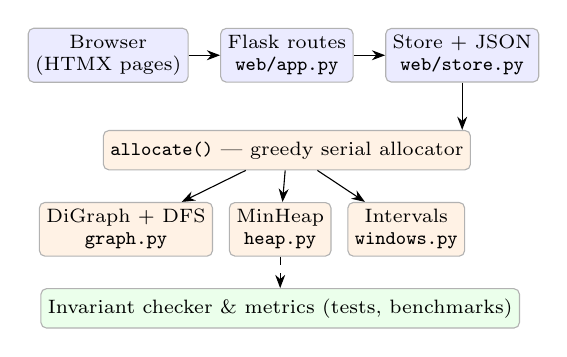
\begin{tikzpicture}[font=\scriptsize, box/.style={draw=gray!60, rounded corners=2pt, fill=#1, minimum height=5mm, inner sep=2.5pt, align=center}, >=Stealth]
\node[box=blue!8] (ui) {Browser\\(HTMX pages)};
\node[box=blue!8, right=4mm of ui] (app) {Flask routes\\\texttt{web/app.py}};
\node[box=blue!8, right=4mm of app] (store) {Store + JSON\\\texttt{web/store.py}};
\node[box=orange!10, below=6mm of app, minimum width=46mm] (alloc) {\texttt{allocate()} --- greedy serial allocator};
\node[box=orange!10, below left=4mm and -14mm of alloc] (graph) {DiGraph + DFS\\\texttt{graph.py}};
\node[box=orange!10, right=2mm of graph] (heap) {MinHeap\\\texttt{heap.py}};
\node[box=orange!10, right=2mm of heap] (win) {Intervals\\\texttt{windows.py}};
\node[box=green!8, below=4mm of heap, minimum width=46mm] (chk) {Invariant checker \& metrics (tests, benchmarks)};
\draw[->] (ui) -- (app); \draw[->] (app) -- (store);
\draw[->] (store.south) -- (store.south |- alloc.north);
\draw[->] (alloc) -- (graph); \draw[->] (alloc) -- (heap); \draw[->] (alloc) -- (win);
\draw[->, dashed] (heap) -- (chk);
\end{tikzpicture}
\caption{Architecture. The engine (orange) has no dependencies on the web layer (blue).}
\label{fig:arch}
\end{figure}

\subsection{User Interface and Workflow}
The interface follows the proposal's three-step workflow (Figure~\ref{fig:ui}).
\textbf{Today} is exception-based: a ``needs you'' panel asks yes/no questions (did the
client approve? is this person working today?), completed work and not-yet-actionable gates
are hidden by default, and a bulk-action bar appears only when rows are selected.
\textbf{Plan} shows a one-sentence summary, a per-person timeline, the proposed sequence,
and a plain reason for every task that cannot start (for example ``No continuous 3h slot
for qualified staff''). \textbf{Campaigns} creates all steps, links, skills, and effort
ranges of a campaign from a template. A ``client asked for changes'' action closes the
review gate and appends a new revision task and review gate, so revisions never reopen
finished work or create cycles.

\begin{figure}[t]
\centering
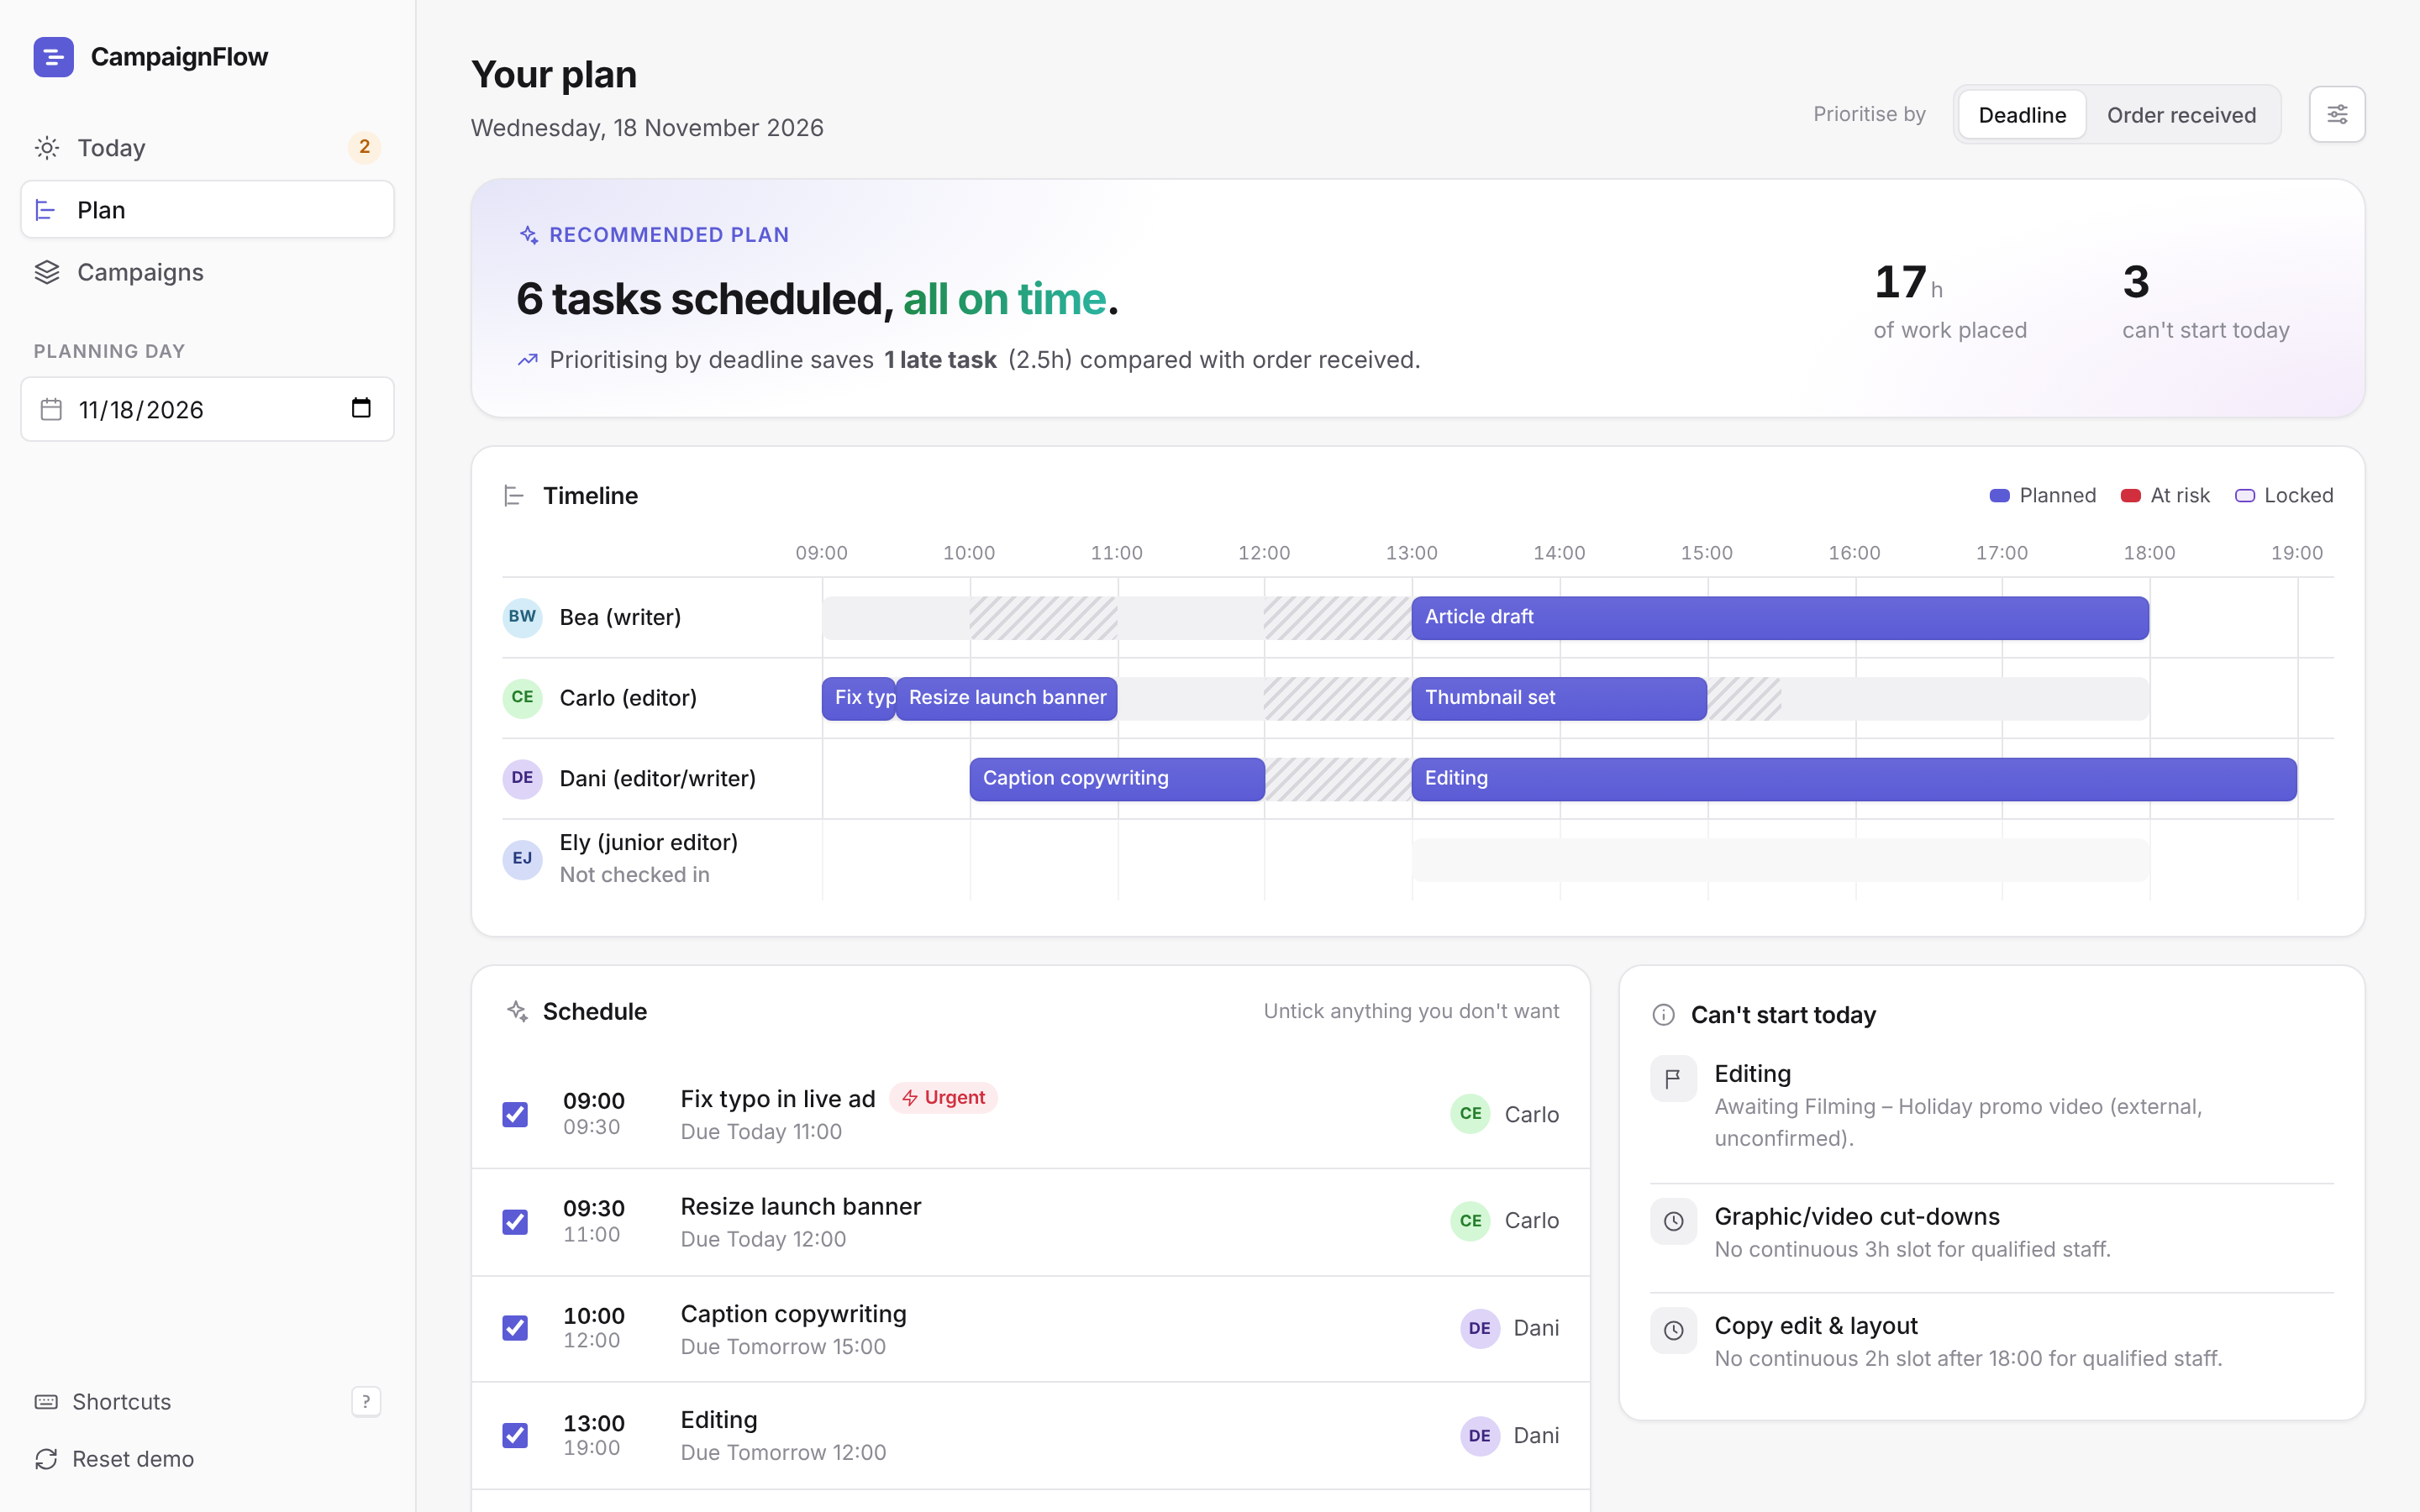
\includegraphics[width=\linewidth]{figures/plan.png}
\caption{The Plan page: summary and policy comparison, per-person timeline with meetings
hatched, proposed sequence, and reasons for unscheduled work.}
\label{fig:ui}
\end{figure}

\subsection{Data Input, Output, and Error Handling}
Inputs are entered through forms or templates and stored in one JSON file written
atomically (write to a temporary file, then rename). Times are converted to integer minutes
from midnight of the planning day so interval arithmetic is exact. Errors are separated into
two classes (Table~\ref{tab:errors}). \emph{Hard errors} make any schedule untrustworthy, so
allocation stops and the page lists every problem. \emph{Soft gaps} only hold back the
affected task, which is reported with its reason while the rest of the day is still
planned. Form input errors are returned as messages instead of exceptions, and every state
change increments a version number so a recommendation computed from stale inputs cannot be
accepted.

\begin{table}[t]
\centering
\caption{Error handling.}
\label{tab:errors}
\small
\begin{tabular}{@{}p{0.43\linewidth}p{0.5\linewidth}@{}}
\toprule
\textbf{Condition} & \textbf{Behaviour} \\
\midrule
Circular dependency & Hard error; the loop is named, e.g.\ ``Article draft $\to$ Copy edit $\to$ Article draft'' \\
Unknown prerequisite, min $>$ max effort & Hard error, allocation stops \\
Overlapping or out-of-hours commitment & Hard error until reviewed or unlocked \\
Missing estimate or skill & Task held back, ``needs information'' \\
Availability not confirmed today & Person excluded, tasks explain why \\
No continuous slot & Task reported as ``no slot today'' \\
Stale recommendation & Accept refused, refreshed plan shown \\
\bottomrule
\end{tabular}
\end{table}

\subsection{Key Design Decisions}
\begin{itemize}
\item \textbf{Reserve the upper effort estimate.} Plans are conditional on estimates being
  upper bounds; the interface never presents them as promised finish times.
\item \textbf{Gates never auto-release.} Dependent work waits for manager confirmation,
  matching the proposal's rule that expected approval dates do not release work.
\item \textbf{Same-day release of internal prerequisites (configurable).} An internal task
  may start once its prerequisite is \emph{planned} to finish. This deviates from the
  proposal, which released work only after confirmed completion; we made it a visible
  setting because the strict rule left most chained work unscheduled for the day.
\item \textbf{Policies are heap keys.} The deadline rule and the entry-order baseline share
  the same allocator, feasibility checks, and tie-breaks; only the key function differs,
  so measured differences come from the ordering policy alone.
\item \textbf{Independent invariant checker.} Hard constraints are re-derived from raw inputs
  in a separate module, so an allocator bug cannot validate itself.
\end{itemize}

% =====================================================================
\section{Algorithms and Data Structures}
% =====================================================================
Throughout, $n$ is the number of tasks, $e$ the number of dependency links, $s$ the number
of staff, and $w$ the number of free intervals per person.

\subsection{Directed Graph with Adjacency Lists}
Each task or gate is a vertex; an edge $u \to v$ means $u$ must finish before $v$. We store
both successor and predecessor lists in dictionaries of lists. Successors answer ``what does
finishing $u$ release?'' and predecessors answer ``what is $v$ waiting on?'', each in time
proportional to the answer. A matrix would cost $\Theta(n^2)$ space for a graph whose
average out-degree in our workloads is below one.

\subsection{Array Min-Heap Priority Queue}
Ready tasks wait in a binary min-heap stored in a Python list, with children of index $i$ at
$2i{+}1$ and $2i{+}2$. Each entry carries its key, computed once on insertion. The
deadline policy uses the key (urgency rank, deadline, task ID) and the baseline uses
(urgency rank, entry order, task ID); task IDs make ties deterministic. The initial ready set
is built bottom-up in $O(n)$, and tasks released later are pushed in $O(\log n)$. Re-sorting
the ready list after every placement would cost $O(n \log n)$ per placement instead.

\subsection{Iterative DFS Cycle Detection}
Before any allocation, a depth-first search colours vertices white (unvisited), gray (on the
current path), or black (finished). Reaching a gray vertex means an edge points back into
the current path, so the graph has a cycle. We use an explicit stack of
\textit{(vertex, next-child index)} frames instead of recursion, so a chain of 5{,}000 tasks (five times Python's default recursion limit) is checked without
error; a regression test covers this. Parent pointers
recover the exact loop for the error message.

\begin{lstlisting}[style=pseudo]
color[v] = WHITE for every v
for each root with color[root] = WHITE
  color[root] = GRAY; push (root, 0)
  while stack not empty
    (v, i) = top of stack
    if i < |succ(v)|
      top.i = i + 1; w = succ(v)[i]
      if color[w] = WHITE: color[w] = GRAY; parent[w] = v; push (w, 0)
      else if color[w] = GRAY: return path(parent, v, w)   // cycle
    else color[v] = BLACK; pop
return none
\end{lstlisting}

\subsection{Greedy Priority-Based Allocation}
The allocator is a serial schedule-generation scheme~\cite{kolisch1996}. Free windows for
each person are their working hours minus meetings, absences, existing commitments, and the
past. Each task keeps a count of unresolved prerequisites; a task enters the heap when its
count reaches zero.

\begin{lstlisting}[style=pseudo]
free[p] = windows(p) - meetings(p) - commitments(p) - [0, now)
heap = heapify({t : t pending and unresolved[t] = 0})
while heap not empty
  t = heap.pop()                    // most urgent, earliest deadline
  if t lacks estimate/skill/qualified staff: report reason; continue
  best = none
  for each confirmed person p with skill(t), in (#skills, id) order
    if longest(free[p]) < effort_max(t): continue           // prune
    start = earliest_fit(free[p], release[t], effort_max(t))
    best = min(best, (start + effort_max(t), #skills(p), id(p)))
    if start = release[t]: break                           // prune
  if best = none: report "no continuous slot"; continue
  reserve(free[p*], start, finish); record assignment
  for each successor v of t
    unresolved[v] -= 1; release[v] = max(release[v], finish)
    if unresolved[v] = 0: heap.push(v)
\end{lstlisting}

Ties between people are broken by earliest finish, then fewer declared skills (keeping
generalists free), then ID. A task that cannot be placed does not block lower-priority work.
The two pruning rules never change the result: a person whose longest free block is too short
cannot fit the task, and once someone can start at the earliest possible time no later
candidate, scanned in tie-break order, can do better.

\subsection{Free-Window Interval Operations}
Free time is a sorted list of disjoint half-open intervals. Subtraction is a single merge-like
pass; \texttt{earliest\_fit} scans intervals in order and returns the first start that leaves
a continuous gap of the required length; \texttt{reserve} splits one interval into at most
two.

% =====================================================================
\section{Implementation}
% =====================================================================
The engine (about 1{,}000 lines in \texttt{campaignflow/core}) has no imports outside the Python
standard library. Table~\ref{tab:modules} lists the modules. The web layer adds Flask
routes, Jinja templates, a design system with dark mode, and HTMX for in-place updates
(about 2{,}600 lines including templates, CSS, and JavaScript).

\begin{table}[t]
\centering
\caption{Engine modules.}
\label{tab:modules}
\small
\begin{tabular}{@{}ll@{}}
\toprule
\textbf{Module} & \textbf{Responsibility} \\
\midrule
\texttt{models.py} & Task, Staff, Commitment, Plan records \\
\texttt{graph.py} & DiGraph, iterative DFS, downstream search \\
\texttt{heap.py} & Array min-heap with key function \\
\texttt{windows.py} & Interval subtract / fit / reserve \\
\texttt{validate.py} & Hard-error checks before allocation \\
\texttt{policy.py} & Deadline and entry-order heap keys \\
\texttt{allocator.py} & Greedy serial allocation and reasons \\
\texttt{invariants.py} & Independent hard-constraint checker \\
\texttt{metrics.py} & Lateness summary and duration replay \\
\bottomrule
\end{tabular}
\end{table}

The heap's sift-down moves a hole down the tree instead of swapping at every level, which
halves the number of list writes:

\begin{lstlisting}
def _sift_down(self, i):
    data, n, entry = self._data, len(self._data), self._data[i]
    while True:
        child = 2 * i + 1
        if child >= n:
            break
        right = child + 1
        if right < n and data[right][0] < data[child][0]:
            child = right
        if data[child][0] < entry[0]:
            data[i] = data[child]   # move child up into the hole
            i = child
        else:
            break
    data[i] = entry
\end{lstlisting}

The allocator releases successors as soon as a task is placed (with same-day release),
so readiness is maintained incrementally in $O(e)$ total instead of re-scanning all tasks:

\begin{lstlisting}
def resolve(tid, finish):
    for v in graph.successors(tid):
        unresolved[v] -= 1
        if finish > release[v]:
            release[v] = finish
        if unresolved[v] == 0 and is_candidate(tasks[v]):
            heap.push(tasks[v])
\end{lstlisting}

The web layer stores ISO dates and hours, and converts them to engine minutes in one
function (\texttt{engine\_inputs}). Accepting a plan checks the version number the
recommendation was computed from:

\begin{lstlisting}
def accept(st, task_ids, version):
    if version != st["version"]:
        raise InputError("Inputs changed since this recommendation "
                         "was made. Review the refreshed recommendation.")
\end{lstlisting}

% =====================================================================
\section{Testing Procedures and Results}
% =====================================================================
The suite contains 215 automated tests (pytest), all passing (Table~\ref{tab:tests}).

\begin{table}[t]
\centering
\caption{Test suite.}
\label{tab:tests}
\small
\begin{tabular}{@{}p{0.52\linewidth}rp{0.3\linewidth}@{}}
\toprule
\textbf{Category} & \textbf{Tests} & \textbf{Examples} \\
\midrule
Data structures & 13 & heap vs.\ \texttt{heapq} on 5{,}000 random ops; cycle path; 5k-node chain \\
Allocator behaviour & 25 & proposal Table~1; gates; locks; tie-breaks; reasons \\
Randomized invariants & 160 & 40 seeds $\times$ 2 policies $\times$ 2 release modes \\
Web store and routes & 17 & templates; stale accept; revision rounds; HTMX partial \\
\midrule
Total & 215 & all pass in $<$1\,s \\
\bottomrule
\end{tabular}
\end{table}

\paragraph{Unit tests.} The heap is checked against Python's \texttt{heapq} on 5{,}000
random push/pop operations, verifying the heap property after each one. Interval subtraction
is checked against a minute-by-minute brute force on 300 random cases.

\paragraph{Behavioural tests.} The worked example from the proposal is a regression test:
with one editor available 09:00--12:00, the deadline rule schedules ``Edit B'' (due 10:00)
then ``Edit A'' (due 12:00), while entry order makes Edit B finish at 12:00, two hours late.
Other tests cover gate release, committed work, missing information, and validation errors.

\paragraph{Randomized invariants.} For 40 generated workloads (60--255 tasks, varying load,
dependency density, and fragmented windows), every fourth proposal is locked and the day is
replanned around it. The independent checker then verifies: no overlap per person, every
placement inside working hours minus meetings, skill match, reserved length equals the upper
estimate, no gate-dependent work before confirmation, prerequisites finish before dependents
start, locked commitments unchanged, and every pending task either assigned or explained.
A mutation test confirms the checker rejects injected overlaps and skill mismatches.

\paragraph{Bugs found.} Two defects were found and fixed with regression tests. (1) If a
committed task was later marked done, its successors were released twice, which could start
a task before its remaining prerequisite. (2) An early benchmark harness compared schedules
using a dictionary keyed by both \texttt{False} and \texttt{0}, which Python treats as the
same key; the harness, not the scheduler, was at fault.

% =====================================================================
\section{Complexity Analysis}
% =====================================================================
\subsection{Theoretical Bounds}
Table~\ref{tab:complexity} summarizes each operation. Validation is linear in the graph,
dominated by the DFS. In \texttt{allocate}, every task is pushed and popped at most once
($O(n \log n)$), every edge is resolved once ($O(e)$), and each popped task scans its
qualified staff, each scan costing $O(w)$ for \texttt{earliest\_fit}, giving $O(n\,s\,w)$
in the worst case. Pruning lowers the average but not the bound.

\begin{table}[t]
\centering
\caption{Time and space complexity.}
\label{tab:complexity}
\small
\begin{tabular}{@{}lll@{}}
\toprule
\textbf{Operation} & \textbf{Time} & \textbf{Space} \\
\midrule
Graph build & $O(n + e)$ & $O(n + e)$ \\
DFS cycle check & $O(n + e)$ & $O(n)$ \\
Heap push / pop & $O(\log n)$ & $O(n)$ \\
Heapify & $O(n)$ & --- \\
Interval subtract & $O(w + c\log c)$ & $O(w)$ \\
\texttt{earliest\_fit}, \texttt{reserve} & $O(w)$ & $O(w)$ \\
\texttt{validate} & $O(n + e + C\log C)$ & $O(n + e)$ \\
\texttt{allocate} & $O(n\log n + e + n\,s\,w)$ & $O(n + e + s\,w)$ \\
\bottomrule
\end{tabular}
\end{table}

\subsection{Empirical Results}
We timed validation and allocation separately with \texttt{perf\_counter\_ns}~\cite{python-perf},
ten fresh workloads per size, excluding generation, copying, and correctness checks.
The generator sizes the team to the workload (load factor 1.2), so $s$ grows with $n$.
Figure~\ref{fig:scaling} shows the results. On a log-log fit for $n \ge 1{,}000$, allocation
time grows with slope 0.96 against $n \cdot s$, which confirms the $O(n\,s\,w)$ term
dominates; because $s \propto n$ here, it appears as roughly $n^{1.9}$ against $n$ alone.
Validation stays close to linear and peak allocation memory grows with slope 1.02.
For an agency-sized day of 250 tasks and 38 staff, validation took 0.20\,ms and allocation
1.66\,ms; at 10{,}000 tasks and 1{,}480 staff they took 15\,ms and 1.1\,s.

\begin{figure}[t]
\centering
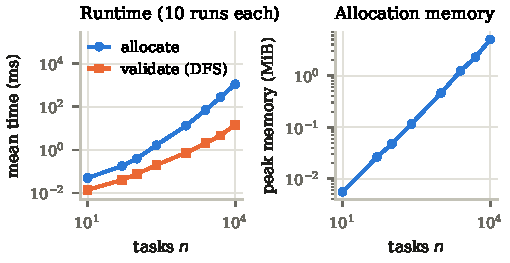
\includegraphics[width=\linewidth]{figures/scaling.pdf}
\caption{Runtime and memory against workload size (log-log). Allocation grows linearly in
tasks $\times$ staff (slope 0.96) and memory linearly in tasks (slope 1.02).}
\label{fig:scaling}
\end{figure}

Table~\ref{tab:pruning} isolates the two pruning rules. The schedules were asserted identical,
and the rules saved 22--27\% of allocation time.

\begin{table}[t]
\centering
\caption{Allocation time with and without pruning (mean of 3 runs, identical output).}
\label{tab:pruning}
\small
\begin{tabular}{@{}rrrr@{}}
\toprule
\textbf{Tasks} & \textbf{Naive (ms)} & \textbf{Pruned (ms)} & \textbf{Speedup} \\
\midrule
1{,}000 & 17.4 & 13.1 & 1.33$\times$ \\
2{,}500 & 92.3 & 71.8 & 1.29$\times$ \\
5{,}000 & 418.4 & 304.4 & 1.37$\times$ \\
10{,}000 & 1{,}446.8 & 1{,}089.5 & 1.33$\times$ \\
\bottomrule
\end{tabular}
\end{table}

% =====================================================================
\section{Schedule Quality}
\label{sec:eval}
% =====================================================================
\paragraph{Policy comparison.} Both policies ran on identical seeded workloads (20 days per
scenario, 250 tasks). Figure~\ref{fig:policies} shows projected lateness under upper
estimates. Deadline-first reduced lateness by 24\% in the baseline scenario, 33\% under
overload, and 22\% with fragmented calendars. The gains shrink to 4\% when dense dependencies
dominate and 7\% when capacity is ample, where order matters less. In a replay where actual
durations ran 20\% longer than sampled estimates, deadline-first produced 36.5 late tasks per
baseline day against 47.0.

\begin{figure}[t]
\centering
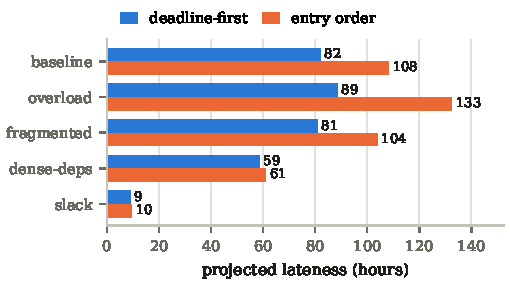
\includegraphics[width=\linewidth]{figures/policies.pdf}
\caption{Projected lateness by scenario (20 synthetic days of 250 tasks each).}
\label{fig:policies}
\end{figure}

\paragraph{Demo day.} The seeded demo agency (4 staff, 7 ready tasks, 6 of which fit the day) shows the same effect
at human scale: the deadline rule places a banner due at 12:00 at 09:30--11:00, while entry
order places it after lunch at 13:00--14:30, 2.5 hours late.

\paragraph{Distance from the optimum.} Because the problem is NP-hard~\cite{blazewicz1983},
the greedy rule is a heuristic. To measure the gap we generated 120 random 7-task days per
regime and fed all $7! = 5{,}040$ task orders through the same serial placement, which
enumerates every schedule the allocator could produce; the best order is the optimum for
this placement model, scored by unplaced tasks, then late tasks, then total lateness.
Figure~\ref{fig:opt} shows how often each policy reached the optimal number of late tasks.
On normal 8-hour days, deadline-first matched it on 53\% of days against 37\% for entry
order, and its mean excess lateness over the optimum was 38 minutes against 81. On
deliberately overloaded 4-hour mornings both rules matched it on only about 30\% of days,
mostly because a different order could have fitted one more task; greedy placement does not
look ahead to pack the day.

\begin{figure}[t]
\centering
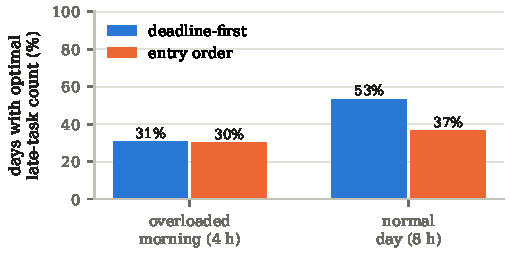
\includegraphics[width=\linewidth]{figures/optimality.pdf}
\caption{Share of small days on which each rule achieved the optimal late-task count
(120 days per regime, brute force over 5{,}040 orders).}
\label{fig:opt}
\end{figure}

% =====================================================================
\section{Limitations and Future Enhancements}
% =====================================================================
\paragraph{Limitations.} All quantitative results use synthetic workloads; they show how the
rules behave, not agency outcomes. The three-person usability study planned in the proposal
was not conducted within the project period, so we make no claims about coordination effort.
Upper estimates can leave capacity unused, urgent work always outranks normal work, and the
greedy rule is not optimal (Section~\ref{sec:eval}). The system depends on timely daily
confirmation and does not coordinate filming resources or predict approvals.

\paragraph{Future enhancements.}
\begin{itemize}
\item \textbf{Faster staff search.} Keep each skill's staff in a balanced tree or heap ordered
  by next free time, so a task inspects only candidates that could start earliest. This targets
  the $O(n\,s\,w)$ term that dominates at large team sizes.
\item \textbf{Better schedules.} Use the greedy plan as a starting point for local search
  (swap adjacent tasks, accept improvements) or an exact solver on small days, guided by the
  optimality gap measured above.
\item \textbf{Richer model.} Multi-person tasks, equipment bookings, tasks split across
  non-contiguous windows, and multi-day horizons.
\item \textbf{Learned estimates.} Replace manual effort ranges with ranges learned from logged
  actual durations.
\item \textbf{Production readiness.} A database instead of a JSON file, accounts and roles,
  and an audit log of overrides.
\item \textbf{User evaluation.} Run the planned study with coordinators, measuring setup and
  update time, interpretation accuracy, and overrides.
\end{itemize}

% =====================================================================
\section{Conclusion}
% =====================================================================
CampaignFlow shows how two classic data structures and two classic algorithms fit together
into a useful planning tool: an adjacency-list graph and DFS make dependencies safe, a min-heap
keeps priority decisions cheap, and a greedy serial allocator turns them into a feasible day.
The implementation plans an agency-sized day in about two milliseconds, never violated a hard
constraint in randomized testing, and reduced projected lateness against arrival order in the
constrained scenarios, while the optimality study marks clearly where a smarter search would
help.

\bibliographystyle{ACM-Reference-Format}
\bibliography{references}

\end{document}
